\newpage
\section{Auswertung}
    In den folgenden Kapiteln wurde ein Höhenkalibrierungsfaktor von $\SI{155}{\nano\metre\per\volt}$ verwendet, um von der anliegenden Spannung am z-Achsen-Piezo zu einer Höhe in Nanometern zu wechseln.
    \subsection{Topografie einer Mikrostruktur}
    \label{sec:Mikro}
        In Abbildung \ref{fig:Strain} sind die Rohdaten der AFM-Aufnahme der Kreisstruktur mit und ohne Strain-Gauge-Nachregelung dargestellt.
        \begin{figure}
            \centering
            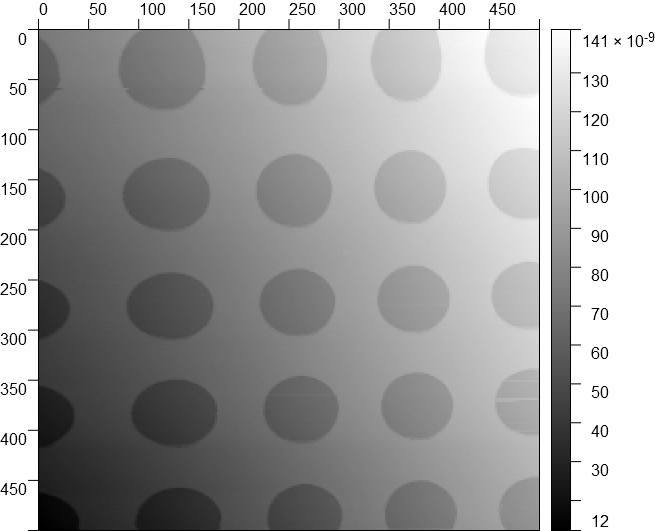
\includegraphics[width = 0.40\textwidth]{pictures/OhneStrain.png}
            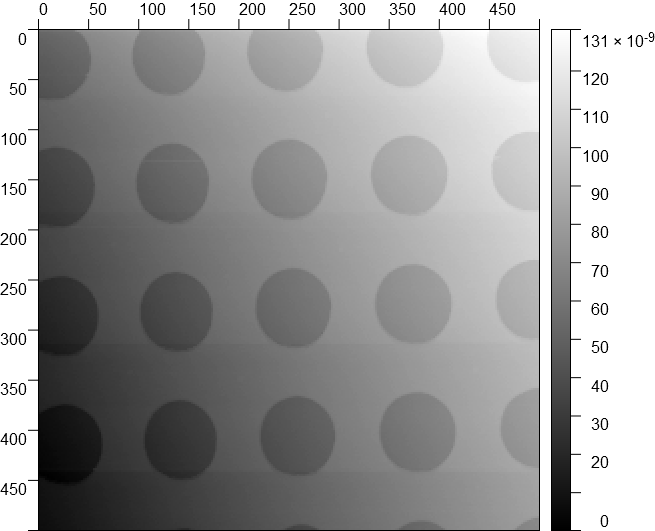
\includegraphics[width = 0.40\textwidth]{pictures/Raw.png}
            \caption{AFM-Aufnahme der Kreisstruktur ohne (links) und mit (rechts) Strain-Gauge-Nachregelung.}
            \label{fig:Strain}    
        \end{figure}
        Die Aufnahme ohne Nachregelung weist eine starke Verzerrung der Kreisstruktur aus, welche bei aktivierter Nachregelung verschwindet.
        Alle im Folgenden gezeigten AFM-Aufnahmen werden aus den Rohaufnahmen gewonnen, indem die Originalbilder invertiert werden, eine Ebenensubstraktion als auch eine Zeilenkorrektur durchgeführt wird und zum Schluss das Bild koloriert wird. Diese Schritte werden mit dem Programm $\textit{Gwiddion}$ \cite{Gwyddion} ausgeführt und der "vorher-nachher Vergleich" ist in Abbildung \ref{fig:VorNach} beispielhaft anhand der Kreisstruktur gezeigt.
        \begin{figure}
            \centering
            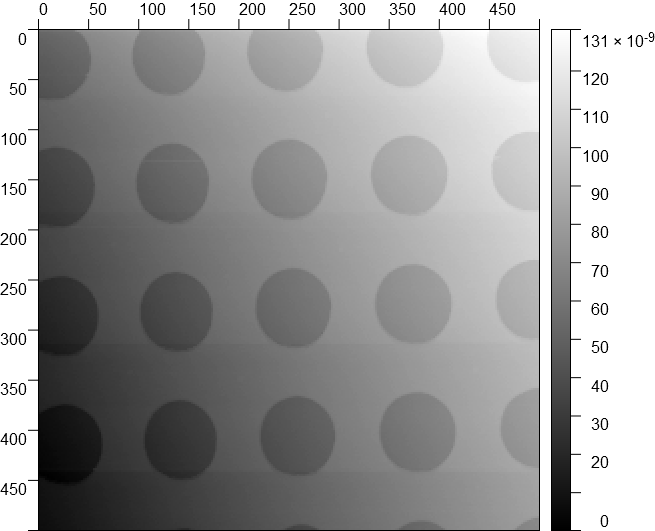
\includegraphics[width = 0.40\textwidth]{pictures/Raw.png}
            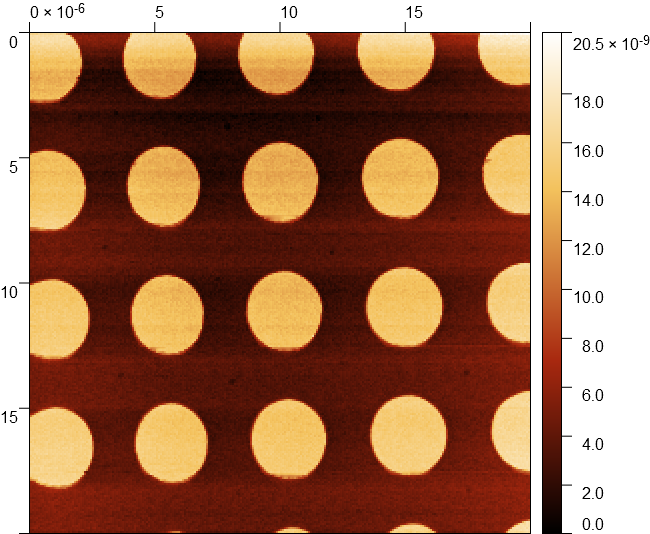
\includegraphics[width = 0.40\textwidth]{pictures/Kreis.png}
            \caption{AFM-Aufnahme der Kreisstruktur vor (links) und nach (rechts) der Bildbearbeitung.}
            \label{fig:VorNach}
        \end{figure}
        Die kolorierten, bearbeiteten Aufnahmen für die Kreis-, Quadrat- und Linienstrukturen sind in Abbildung \ref{fig:2D3D} sowohl zwei- als auch dreidimensional aufgetragen. Da die Aufnahmen vorwärts und rückwärts gemessen ununterscheidbar sind, wird für die Auswertung lediglich eine Messrichtung betrachtet.
        \begin{figure}
            \centering
            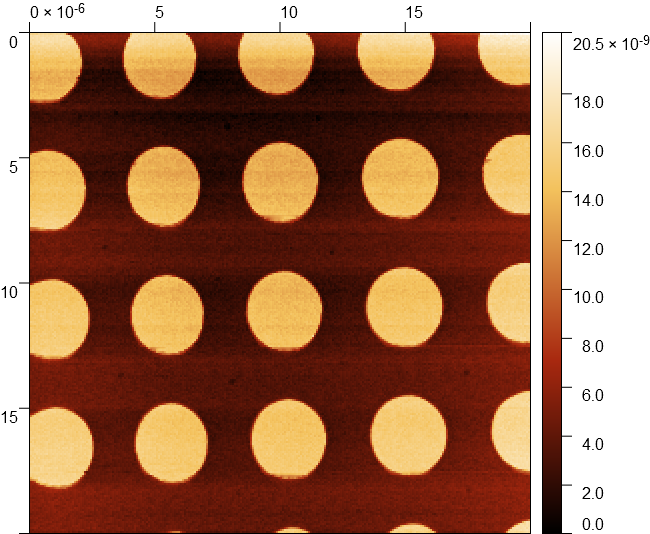
\includegraphics[width = 0.40\textwidth]{pictures/Kreis.png}
            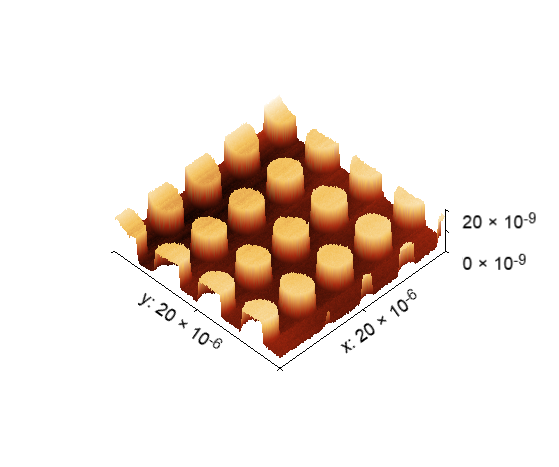
\includegraphics[width = 0.45\textwidth]{pictures/Kreis3D.png}
            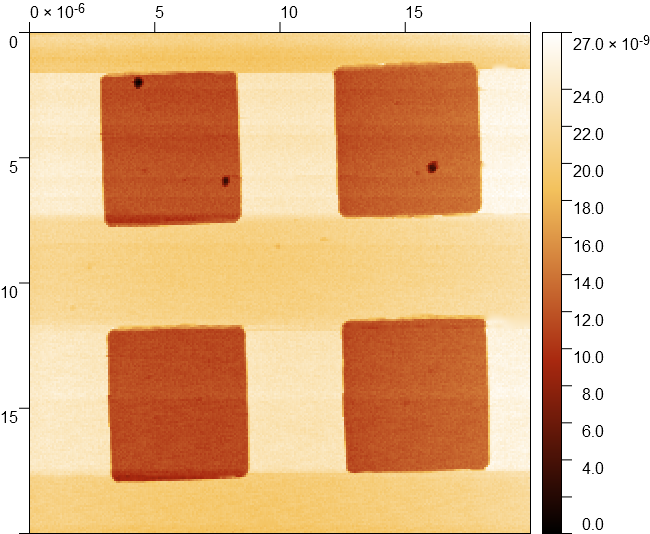
\includegraphics[width = 0.40\textwidth]{pictures/Quadrat.png}
            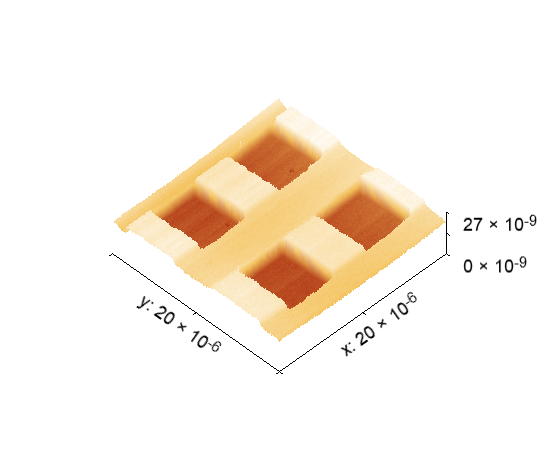
\includegraphics[width = 0.45\textwidth]{pictures/Quadrat3D.png}
            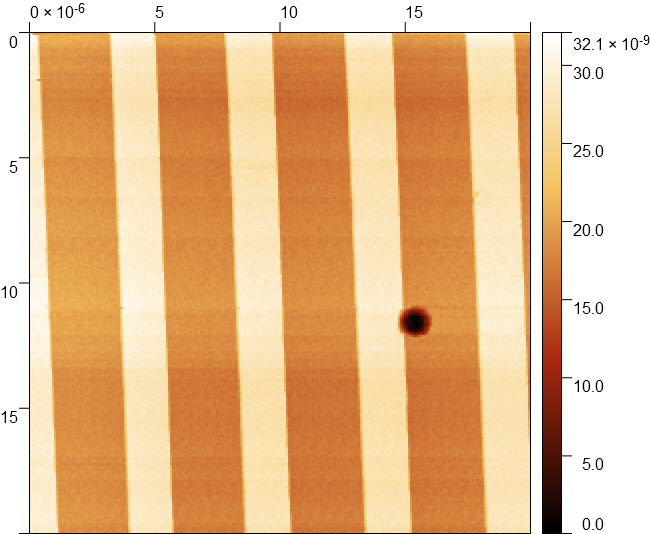
\includegraphics[width = 0.40\textwidth]{pictures/Linie.png}
            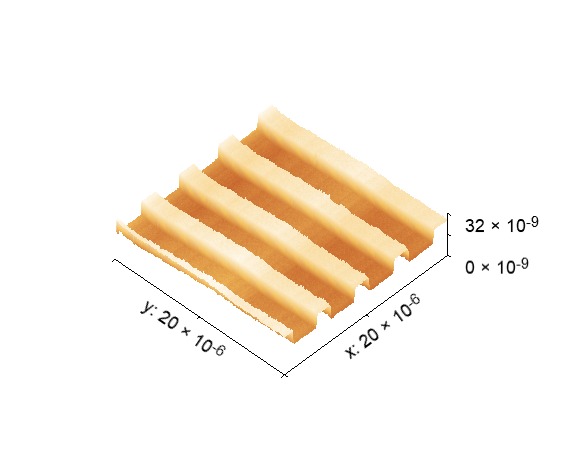
\includegraphics[width = 0.45\textwidth]{pictures/Linie3D.png}
            \caption{AFM-Aufnahmen der Mikrostrukturen als 2D- und 3D-Aufnahmen.}
            \label{fig:2D3D}    
        \end{figure}
        Um die Mikrostrukturen zu vermessen werden Linienprofile entlang bestimmter Richtung betrachtet, wie in Abbildung \ref{fig:Profil} zu sehen ist. Daraus können dann die gesuchten Strukturabmaße bestimmt werden, sowohl in x-y-Richtung parallel zur Probenoberfläche, als auch in z-Richtung - also die Höhe der gemessenen Struktur.
        \begin{figure}
            \centering
            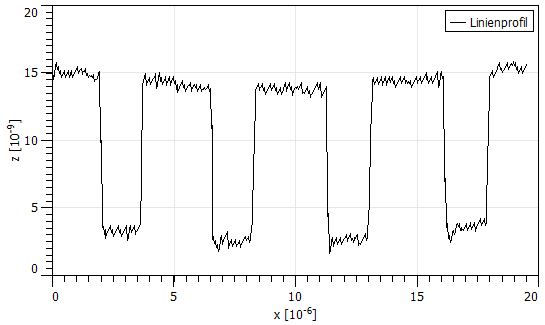
\includegraphics[width = 0.60\textwidth]{pictures/Linienprofil.png}
            \caption{Linienprofil entlang der Kreis-Mikrostruktur. Es wird die Tiefe der Struktur in Abhängigkeit der Position in der x-y-Ebene dargestellt.}
            \label{fig:Profil}    
        \end{figure}
        Es werden für drei Bereiche der Probe die Strukturgröße (Durchmesser bzw. Seitenlänge bzw. Breite) und der Strukturabstand bestimmt. Dabei wird über verschiedene Strukturen aus verschiedenen Linienprofilen gemittelt. Daraus wird durch Addition die mittlere Strukturperiodizität bestimmt, um sie später mit den erwarteten Maßen aus dem Datenblatt vergleichen zu können. Die Werte sind in Tabelle \ref{tab:Werte} aufgelistet.
        \begin{center}
            \captionof{table}{Aus den Linienprofilen bestimmte Strukturabmaße für die drei Bereiche der zu untersuchenden Probe in x- und in y-Richtung.}
            \label{tab:Werte}
            \begin{tabular}{c c c c}
                \toprule
                Mikrostruktur & Strukturgröße / $\mu\text{m}$ & Strukturabstand / $\mu\text{m}$ & Strukturperiodizität / $\mu\text{m}$ \\
                \midrule
                Kreis (X)   & ($3.007\pm 0.044$) & ($1.730\pm 0.023$) & ($4.737\pm 0.067$) \\
                Kreis (Y)   & ($3.163\pm 0.018$) & ($1.917\pm 0.014$) & ($5.080\pm 0.032$) \\
                Quadrat (X) & ($5.672\pm 0.076$) & ($3.765\pm 0.025$) & ($9.437\pm 0.101$) \\
                Quadrat (Y) & ($6.060\pm 0.025$) & ($4.095\pm 0.025$) & ($10.155\pm 0.050$) \\
                Streifen (X)& ($1.840\pm 0.034$) & ($2.900\pm 0.026$) & ($4.740\pm 0.060$) \\
                \bottomrule
            \end{tabular}
        \end{center}
        \FloatBarrier
    \subsection{Topografie einer CD, DVD und Blu-Ray}
        Die AFM-Aufnahmen der drei verschiedenen Datenträger werden wie oben beschrieben bearbeitet und sind in Abbildung \ref{fig:CDB} in zwei bzw. drei Dimensionen dargestellt.
        \begin{figure}
            \centering
            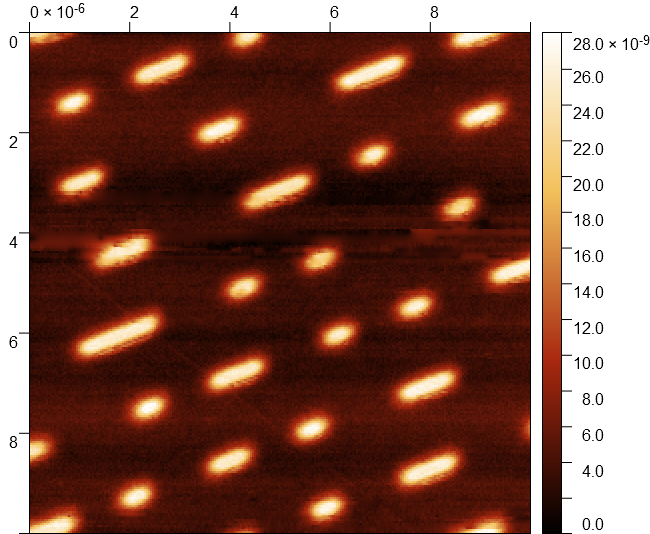
\includegraphics[width = 0.40\textwidth]{pictures/CD.png}
            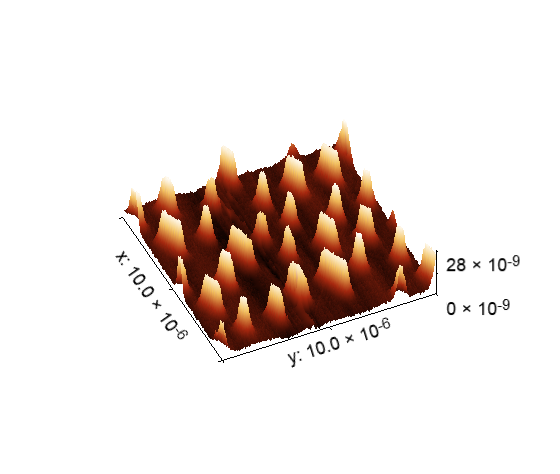
\includegraphics[width = 0.45\textwidth]{pictures/CD3D.png}
            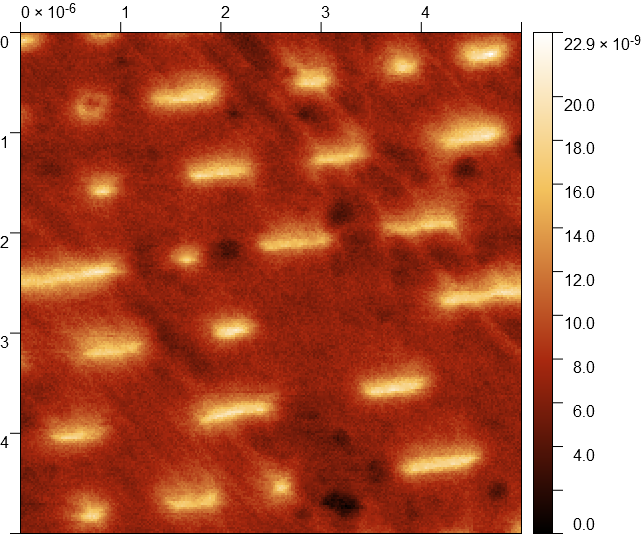
\includegraphics[width = 0.40\textwidth]{pictures/DVD.png}
            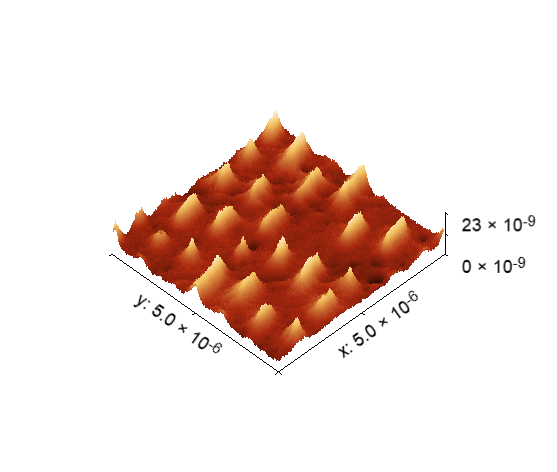
\includegraphics[width = 0.45\textwidth]{pictures/DVD3D.png}
            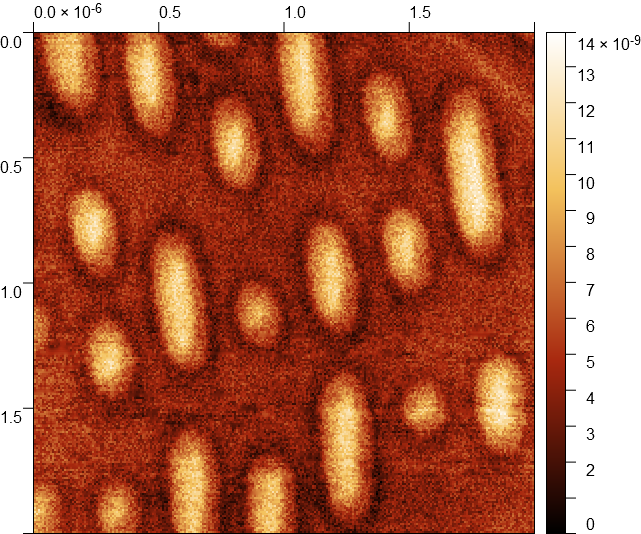
\includegraphics[width = 0.40\textwidth]{pictures/BluRay.png}
            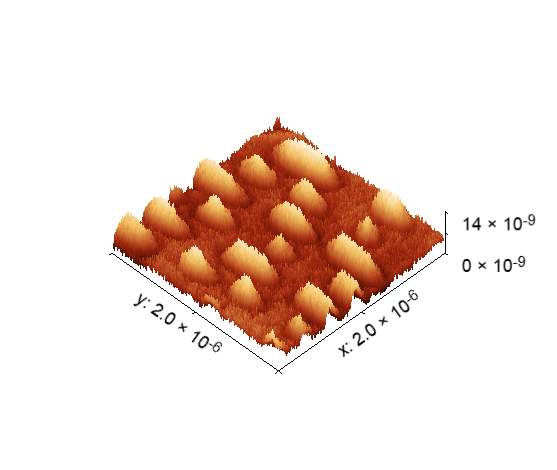
\includegraphics[width = 0.45\textwidth]{pictures/BluRay3D.png}
            \caption{AFM-Aufnahmen der CD (oben), DVD (mitte) und Blu-ray (unten) Proben als 2D- und 3D-Aufnahmen.}
            \label{fig:CDB}    
        \end{figure}
        Auch hier wirde die Profilfunktion benutzt um die Proben zu vermessen. Es werden so die Spurbreite, der Spurabstand, die minimale und maximale sichtbare Pitlänge und die Pittiefe bestimmt. Dazu wird über mehrere Linienprofile und mehrere Pits gemittelt und das Ergebnis der Messungen und Tabelle \ref{tab:Pits} aufgetragen.
        \begin{center}
            \captionof{table}{Gemessene Abmaße der drei untersuchten optischen Datenträger.}
            \label{tab:Pits}
            \begin{tabular}{c c c c}
                \toprule
                Datenträger & CD & DVD & BluRay \\
                \midrule
                Spurbreite / $\mu\text{m}$    & ($0.424\pm 0.024$) & ($0.218\pm 0.007$) & ($0.158\pm 0.002$) \\
                Spurabstand / $\mu\text{m}$   & ($1.123\pm 0.032$) & ($0.623\pm 0.053$) & ($0.150\pm 0.006$) \\
                min. Pitlänge / $\mu\text{m}$ & ($0.684\pm 0.013$) & ($0.283\pm 0.022$) & ($0.183\pm 0.010$) \\
                max. Pitlänge / $\mu\text{m}$ & ($1.715\pm 0.035$) & ($0.990\pm 0.001$) & ($0.576\pm 0.003$) \\
                Pittiefe / $\text{nm}$        & ($22.141\pm 0.448$)& ($11.753\pm 0.265$) &($8.210\pm 0.211$) \\
                \bottomrule
            \end{tabular}
        \end{center}
        Außerdem wird die maximale Speicherkapazität einer CD bestimmt. Dazu muss als Erstes die gesamte Länge der spiralförmigen Spur bestimmt werden, welche zwischen dem Innenradius $R_I=23\,\text{mm}$ und dem Außenradius $R_A=58.5\,\text{mm}$ der CD verläuft \cite{RadiusCD}. Dazu nähern wir diese als $n$ Kreise an mit einem Abstand untereinander von $d=Spurbreite+Spurabstand=(1.547\pm 0.056)\,\mu\text{m}$, also
        \begin{equation}
            n=\frac{R_A-R_I}{d}=229050 \, .
        \end{equation}
        Für die Spurlänge ergibt sich dann
        \begin{equation}
            L = \sum_{i=0}^{n} 2\pi\left(R_I+i\cdot d\right) = (5876.63 \pm 0.71) \, \text{m} \, .
        \end{equation}
        Wie in der Versuchsanleitung beschrieben, beschreibt der kleinstmögliche Pit die Abfolge"1001" und entspricht 4 Bit. Die minimale gemessene Pitlänge beträgt $p_{min}=0.684\pm 0.013\,\mu\text{m}$. Daraus ergibt sich für die Speicherkapazität der CD
        \begin{equation}
            C_{Speicher} = \frac{L}{p_{min}}\cdot 4\,\text{Bits} \cdot \frac{1\,\text{B}}{8\,\text{Bit}} = (4295.79\pm 81.65)\,\text{MB}
        \end{equation}
        \FloatBarrier
    \subsection{Adhäsionskraft und Elastizitätsmodul}
        In Abbildung \ref{fig:KA} sind die Kraft-Abstands-Kurven für die Edelstahl-, Teflon- und DLC-Probe zu sehen. Da bekannt ist, dass das z-Piezo-Element bei einer
        Maximalspannung von \SI{75}{\volt} um \SI{20}{\micro\metre} ausgelenkt ist, kann die z-Piezo-Spannung in einen Abstand umgerechnet werden, welche auf der x-Achse aufgetragen ist. Der Ursprung dieses Abstandes ist dabei beliebig gesetzt und hängt von der anfänglichen Position der Probe ab. Da im Folgenden nur auf eine Abstandsdifferenz eingegangen wird, spielt das aber keine Rolle. Auf der y-Achse ist gemessene Spannung am Cantilever-Piezo aufgetragen, gibt also ein Maß für die Auslenkung des Cantilevers an.
        Wie in Kapitel \ref{sec:KraftAbstand} beschrieben sind bei einer Annäherung der Probe und Spitze der Snap-In mit anschließender steigender Flanke beobachtbar. Beim Zurückziehen der Probe fällt die Piezospannung am Cantilever wieder ab und sinkt unter die Ruhepoition ab, was auf die Adhäsionskraft zwischen der Spitze und der Probe zurückzuführen ist. Wird diese durch die rücktreibende Kraft des Cantilevers ausgeglichen, kommt es zum Pull-Off und der Cantilever bewegt sich wieder in seine Ruhepostion zurück. (siehe Abbildung \ref{fig:KA})
        \begin{figure}
            \centering
            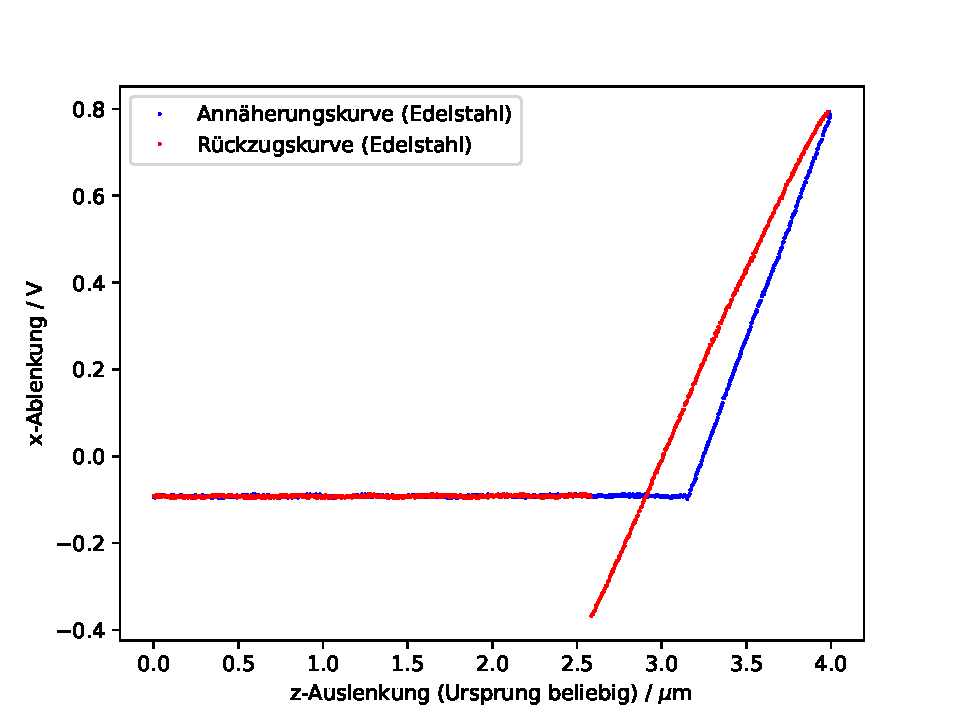
\includegraphics[width = 0.60\textwidth]{pictures/Edelstahl.pdf}
            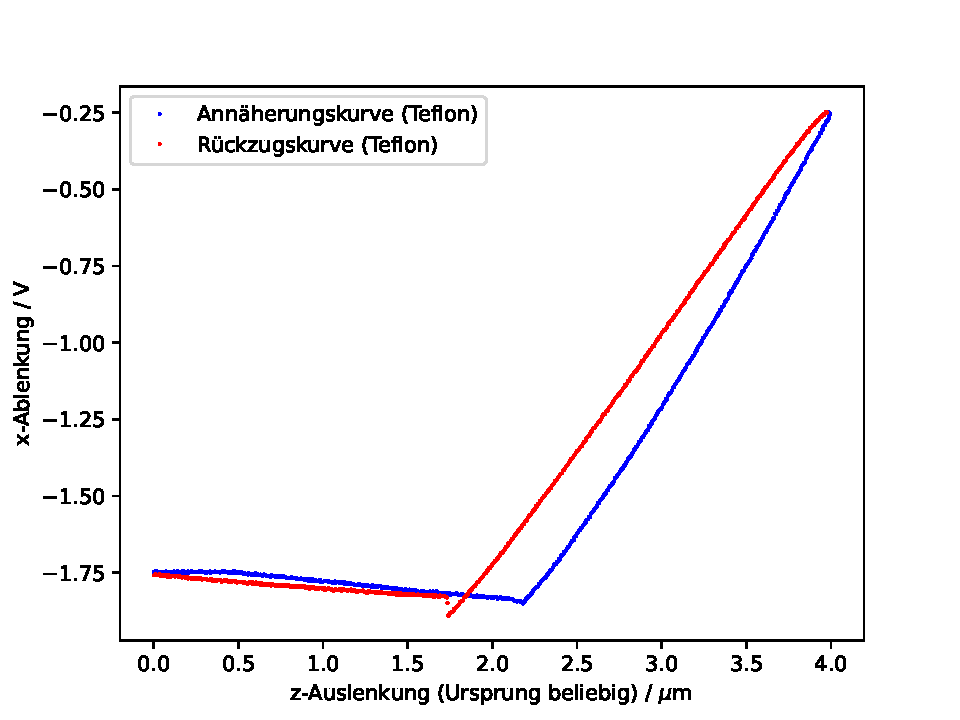
\includegraphics[width = 0.60\textwidth]{pictures/Teflon.pdf}
            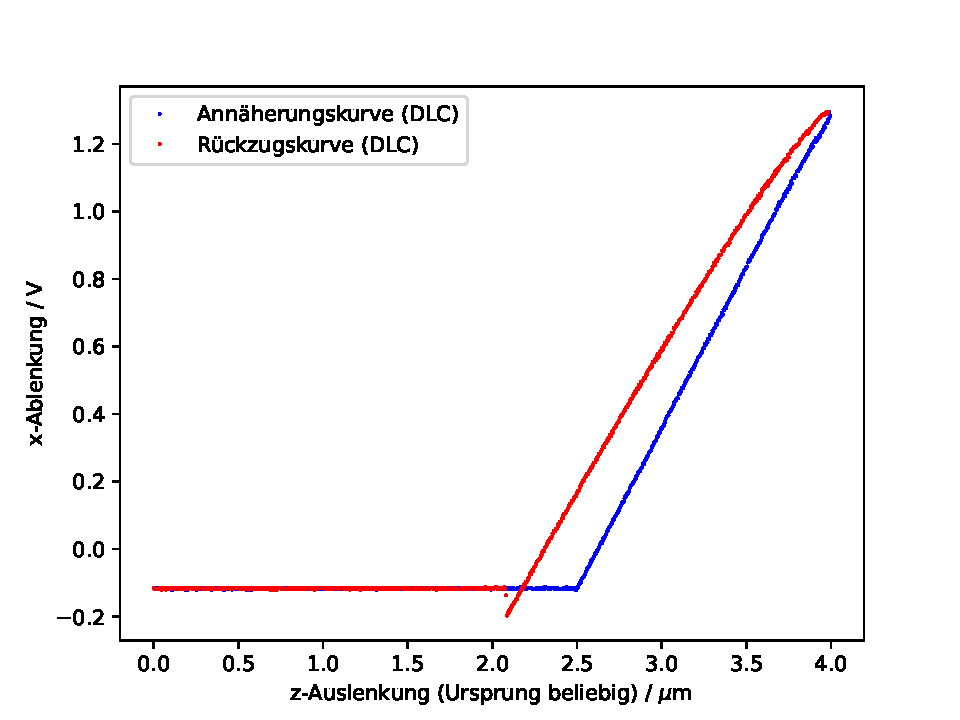
\includegraphics[width = 0.60\textwidth]{pictures/DLC.pdf}
            \caption{Kraft-Abstands-Kurven der drei untersuchten Proben. Die Annäherung und Entfernung von der Probe sind in unterschiedlichen Farben gekennzeichnet.}
            \label{fig:KA}    
        \end{figure}
        Der größere Pull-Off beim Edelstahl ist dabei die Folge einer größeren Adhäsionskraft und die, im Vergleich zu den anderen Proben, flachere Flanke der Teflon-Probe ein Zeichen für eine höhere Elastizität, wie im Folgenden beschrieben ist.

        Die Adhäsionskraft $F_A$ ist die Kraft, die überwunden werden muss, um den Kontakt zwischen Spitze und Probe aufzulösen. Diese kann aus der Abstandsdifferenz $\Delta_{SP}$ zwischen Snap-In und Pull-Off berechnet werden. Es gilt
        \begin{equation}
            F_A = k\cdot\Delta_{SP} \, ,
        \end{equation}
        für die maximale Adhäsionskraft mit der Ferderkonstante $k=\SI{0.2}{\newton\per\metre}$ des Cantilevers. Die Abstandsdifferenzen und die daraus berechneten Adhäsionskräfte für die drei untersuchten Proben sind in Tabelle \ref{tab:AK} aufgelistet.
        \begin{center}
            \captionof{table}{Differenz zwischen Snap-In und Pull-Off und die resultierende Adhäsionskraft der Proben.}
            \label{tab:AK}
            \begin{tabular}{c c c}
                \toprule
                Probe & Diferenz zw. Snap-In und Pull-Off / $\mu\text{m}$ & Adhäsionskraft / $\text{nN}$ \\
                \midrule
                Edelstahl & $0.5749$ & $114.99$\\
                Teflon    & $0.4501$ & $90.03$ \\
                DLC       & $0.4200$ & $84.00$ \\
                \bottomrule
            \end{tabular}
        \end{center}
        Als nächstes wird das Elastizitätsmodul von Teflon bestimmt. Dazu wird folgende Formel \cite{Elastic} betrachtet:
        \begin{equation}
            F_K = \frac{E}{1-\nu^2}\,\frac{2\,\tan(\alpha)}{\pi}\,\delta^2 \qquad
            \label{eqn:FFF}
        \end{equation}
        Diese beschreibt die Kraft $F_K$, welche durch eine kegelförmige Spitze mit Öffnungswinkel $2\alpha$ auf eine Probe mit dem \textit{Young Elastizitätsmodul} $E$ wirkt. $\nu$ ist dabei die materialabhängige \textit{Poisson-Zahl} und $\delta$ beschreibt die Eindringtiefe der Spitze in die Probe. Für die die Elastizität ergibt sich nach umstellen von Formel \ref{eqn:FFF}
        \begin{equation}
            E = \frac{\pi}{2}\left(1-\nu^2\right)\,\frac{1}{\tan(\alpha)}\,\frac{1}{\delta^2}\cdot F_K
            \label{eqn:EEE}
        \end{equation}
        Um die Kraft $F_K$ und die Eindringtiefe $\delta$ zu bestimmen muss die zu untersuchende Teflon-Probe mit einer undeformierbaren Probe - in unserem Fall Edelstahl - verglichen werden. Dazu sind ansteigenden Flanke beim Annäherungsprozess aus den Kraft-Abstand-Kurven für Teflon und Edelstahl in Abbildung \ref{fig:Ela} aufgetragen. Der Snap-In wurde jeweils auf den Ursprung beider Achsen gelegt, um beide Proben vergleichen zu können.
        \begin{figure}
            \centering
            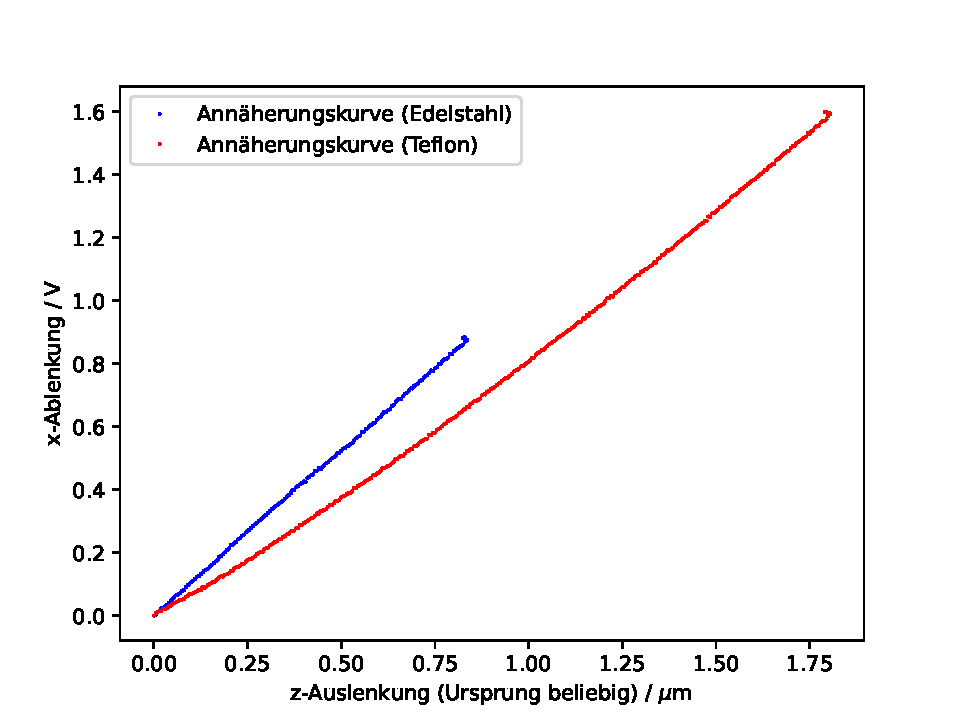
\includegraphics[width = 0.60\textwidth]{pictures/Ursprung.pdf}
            \caption{Annäherungsprozess der Edelstahl- und Teflon-Proben. Die Snap-In Punkte beider Proben sind auf den Ursprung gelegt.}
            \label{fig:Ela}
        \end{figure}
        Als Ausgangspunkt wurde beispielhaft eine z-Auslenkung von $z_{Edelstahl}=\SI{0.75}{\micro\metre}$ der Edelstahl-Probe betrachtet. Die z-Auslenkung der Teflon-Probe, welche die selbe Piezospannung des Cantilevers zur Folge hat liegt bei $z_{Teflon}=\SI{0.97}{\micro\metre}$. Für die Eindringtiefe der Spitze in die Teflon-Probe ergibt sich damit
        \begin{equation}
            \delta = z_{Teflon} - z_{Edelstahl}
            \label{eqn:Eindringen}
        \end{equation}
        und die Kraft des Cantilevers auf die Probe lässt sich berechnen über
        \begin{equation}
            F_K = k\cdot z_{Edelstahl} \, .
            \label{eqn:Druck}
        \end{equation}
        Mit dem halben Öffnungswinkel $\alpha = 10°$ \cite{tu_dortmund_versuchsanleitung_nodate}, der Poissonzahl $\nu = 0.46$ von Teflon \cite{DuPont} und der über \ref{eqn:Eindringen} und \ref{eqn:Druck} berechneten Eindringtiefe $\delta$ und Kraft $F_K$ ergibt sich für das Elastizitätsmodul $E$ mit Formel \ref{eqn:EEE}
        \begin{equation}
            E = \SI{20.8580}{\mega\pascal} \, .
        \end{equation}

